\chapter{Protótipos}

Para elucidar qualquer dúvida, e garantir a satisfação do usuário antes de começar o desenvolviemento, foram criados protótipos dos casos de usos priorizados. Posteriormente os protótipos foram validados juntamente ao cliente, e então seguiu-se para fase de implementação. 

\begin{figure}[H]
  \center
  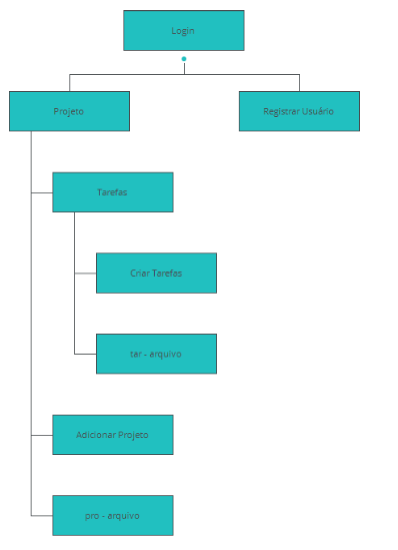
\includegraphics[width=0.7\textwidth]{figuras/Prototipo1}
  \caption{Rastreabilidade Protótipos}
  \label{fig: Rastreabilidade-prototipos}
\end{figure}

\begin{figure}[H]
  \center
  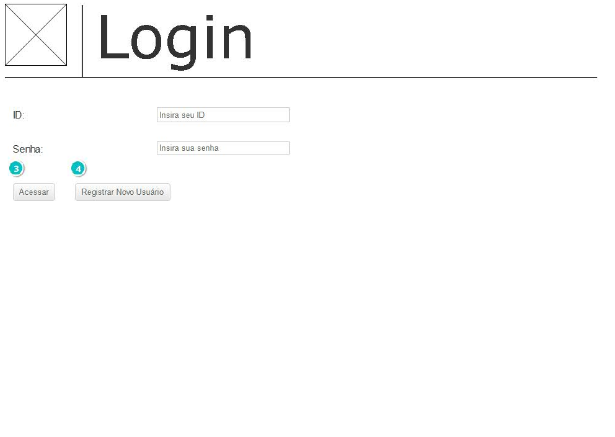
\includegraphics[width=0.9\textwidth]{figuras/Prototipo2}
  \caption{Caso de uso - Logar Usuário}
  \label{fig:uc-logar-usuario}
\end{figure}

\begin{figure}[H]
  \center
  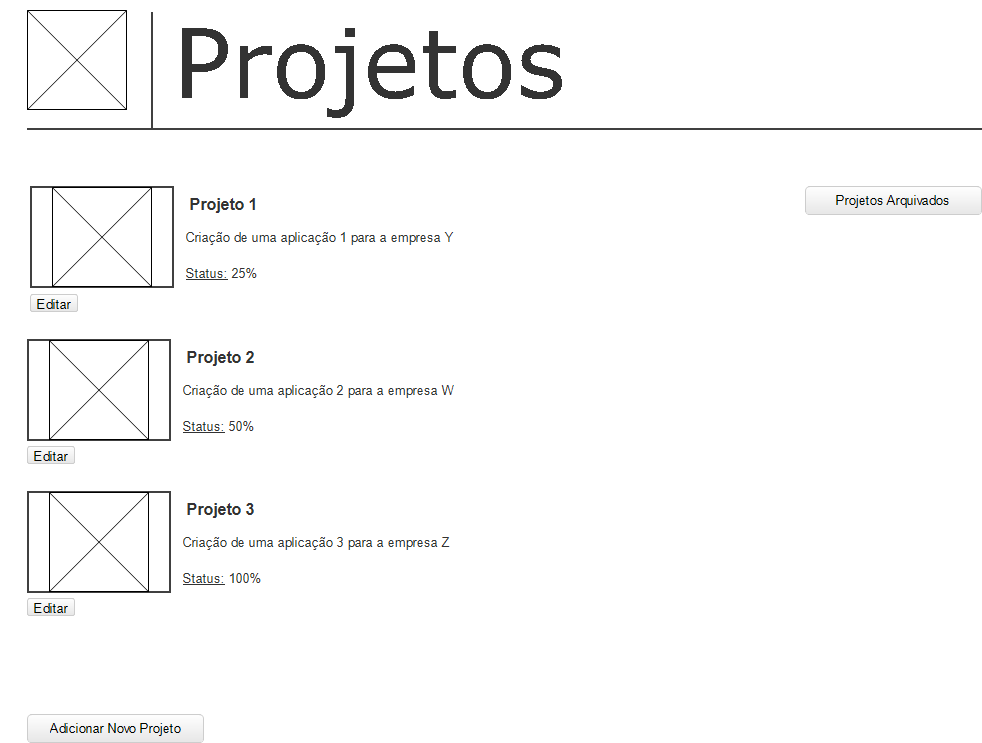
\includegraphics[width=0.9\textwidth]{figuras/Prototipo3}
  \caption{Caso de uso - Visualizar Projeto}
  \label{fig:uc-visualizar-projeto}
\end{figure}

\begin{figure}[H]
  \center
  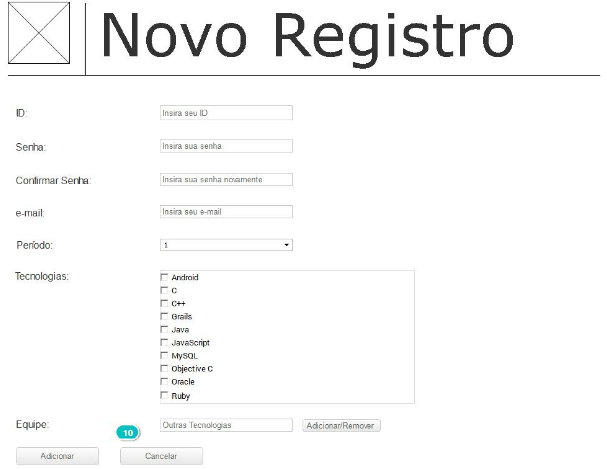
\includegraphics[width=0.9\textwidth]{figuras/Prototipo4}
  \caption{Caso de uso - Cadastrar Usuário}
  \label{fig:uc-cadastrar-usuario}
\end{figure}

\begin{figure}[H]
  \center
  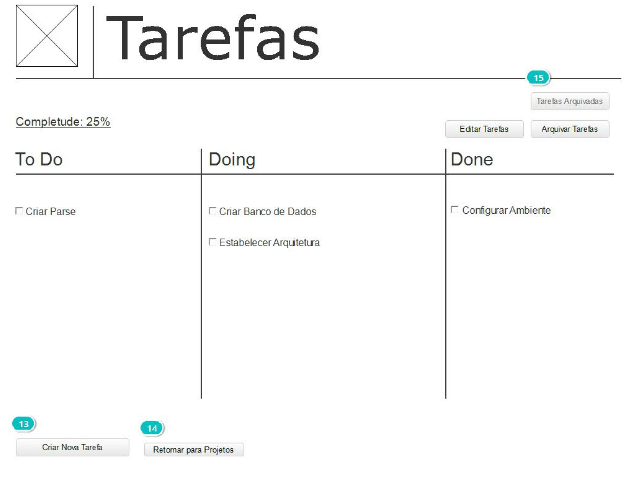
\includegraphics[width=0.9\textwidth]{figuras/Prototipo5}
  \caption{Caso de uso - Visualizar Tarefa}
  \label{fig:uc-visualizar-tarefa}
\end{figure}

\begin{figure}[H]
  \center
  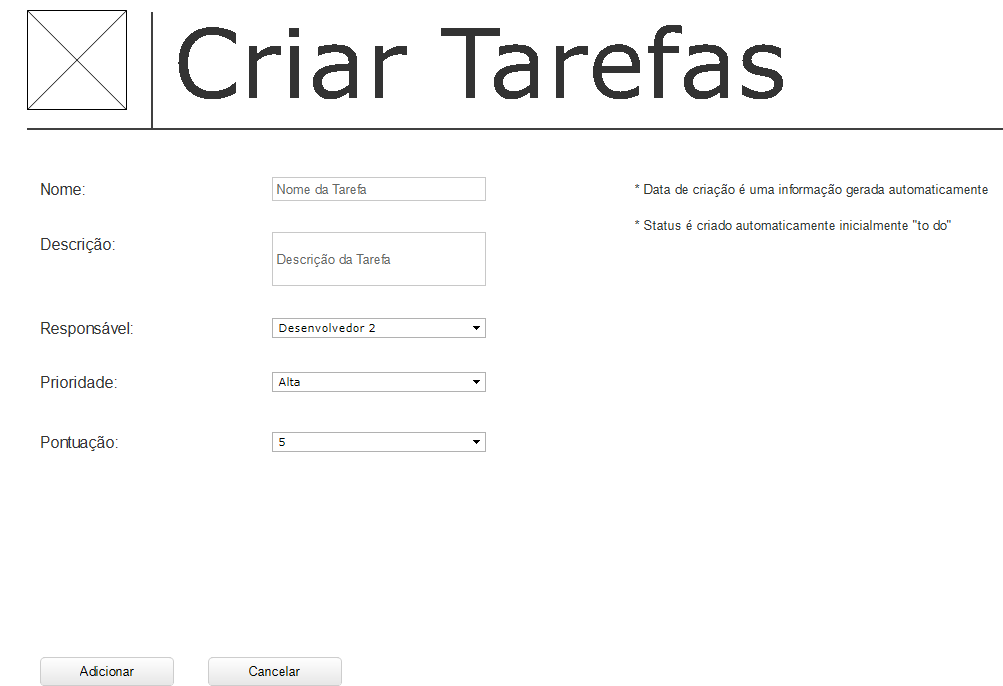
\includegraphics[width=0.9\textwidth]{figuras/Prototipo6}
  \caption{Caso de uso - Cadastrar Tarefa}
  \label{fig:uc-cadastrar-tarefa}
\end{figure}

\begin{figure}[H]
  \center
  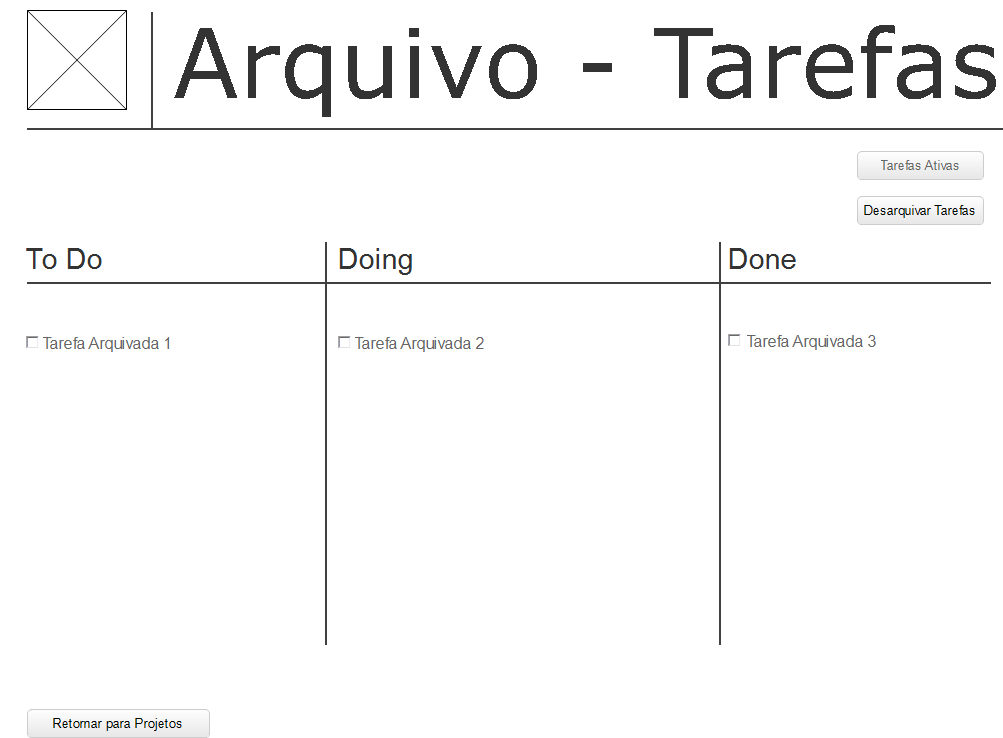
\includegraphics[width=0.9\textwidth]{figuras/Prototipo7}
  \caption{Caso de uso - Arquivar Tarefa}
  \label{fig: uc-arquivar-tarefa}
\end{figure}

\begin{figure}[H]
  \center
  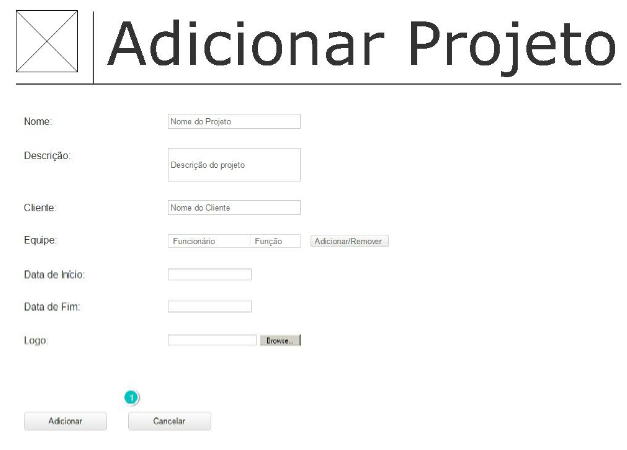
\includegraphics[width=0.9\textwidth]{figuras/Prototipo8}
  \caption{Caso de uso - Adicionar Projeto}
  \label{fig:uc-adicionar-projeto}
\end{figure}

\begin{figure}[H]
  \center
  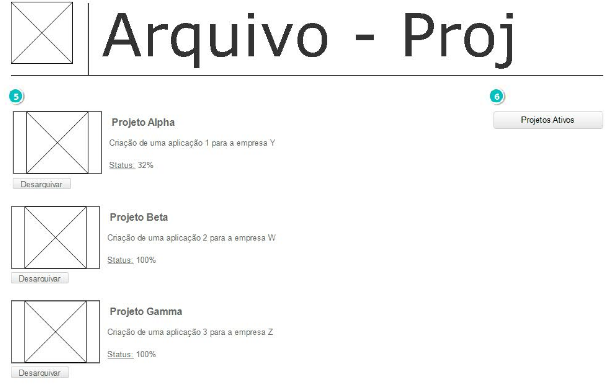
\includegraphics[width=0.9\textwidth]{figuras/Prototipo9}
  \caption{Caso de uso - Arquivar Projeto}
  \label{fig: uc-arquivar-projeto}
\end{figure}

